\documentclass[11pt]{article}
\usepackage[margin=1in]{geometry}
\usepackage[T1]{fontenc}
\usepackage{lmodern}
\usepackage{amsmath,amssymb,amsthm}
\usepackage{graphicx}
\usepackage[hidelinks]{hyperref}
\usepackage{microtype}
\emergencystretch=2em

\newtheorem{theorem}{Theorem}
\newtheorem{lemma}{Lemma}
\newcommand{\R}{\mathbb R}
\newcommand{\eps}{\varepsilon}
\newcommand{\ga}{\gamma_2}
\newcommand{\cL}{\mathcal L}

\title{A parabolic counterexample to the Gaussian Neumann-to-Dirichlet condition}
\author{Run fa\_banach\_001, agent\_lane\_14}
\date{2026-08-09}

\begin{document}
\maketitle

\section*{Status}

\textbf{Candidate counterexample; likely valid, pending human review.}

\section*{Source Question}

The source is Alexander V. Kolesnikov and Emanuel Milman,
\emph{Sharp Poincar\'e-type inequality for the Gaussian measure on the boundary
of convex sets}, arXiv:1601.02925v2 \cite{KM}.  Question 3.4 on page 11 asks
whether condition (3.2) holds for standard Gaussian measure with
\[
 F(v)=\frac1v-(\log I_\gamma)'(v),
 \qquad I_\gamma(v)=\varphi(\Phi^{-1}(v)).
\]
Here is the question in the source.

\begin{center}

\includegraphics[width=0.98\linewidth]{figures/open_problem_crop.png}
\end{center}

Condition (3.2), together with the Neumann problem to which it applies, is:

\begin{center}
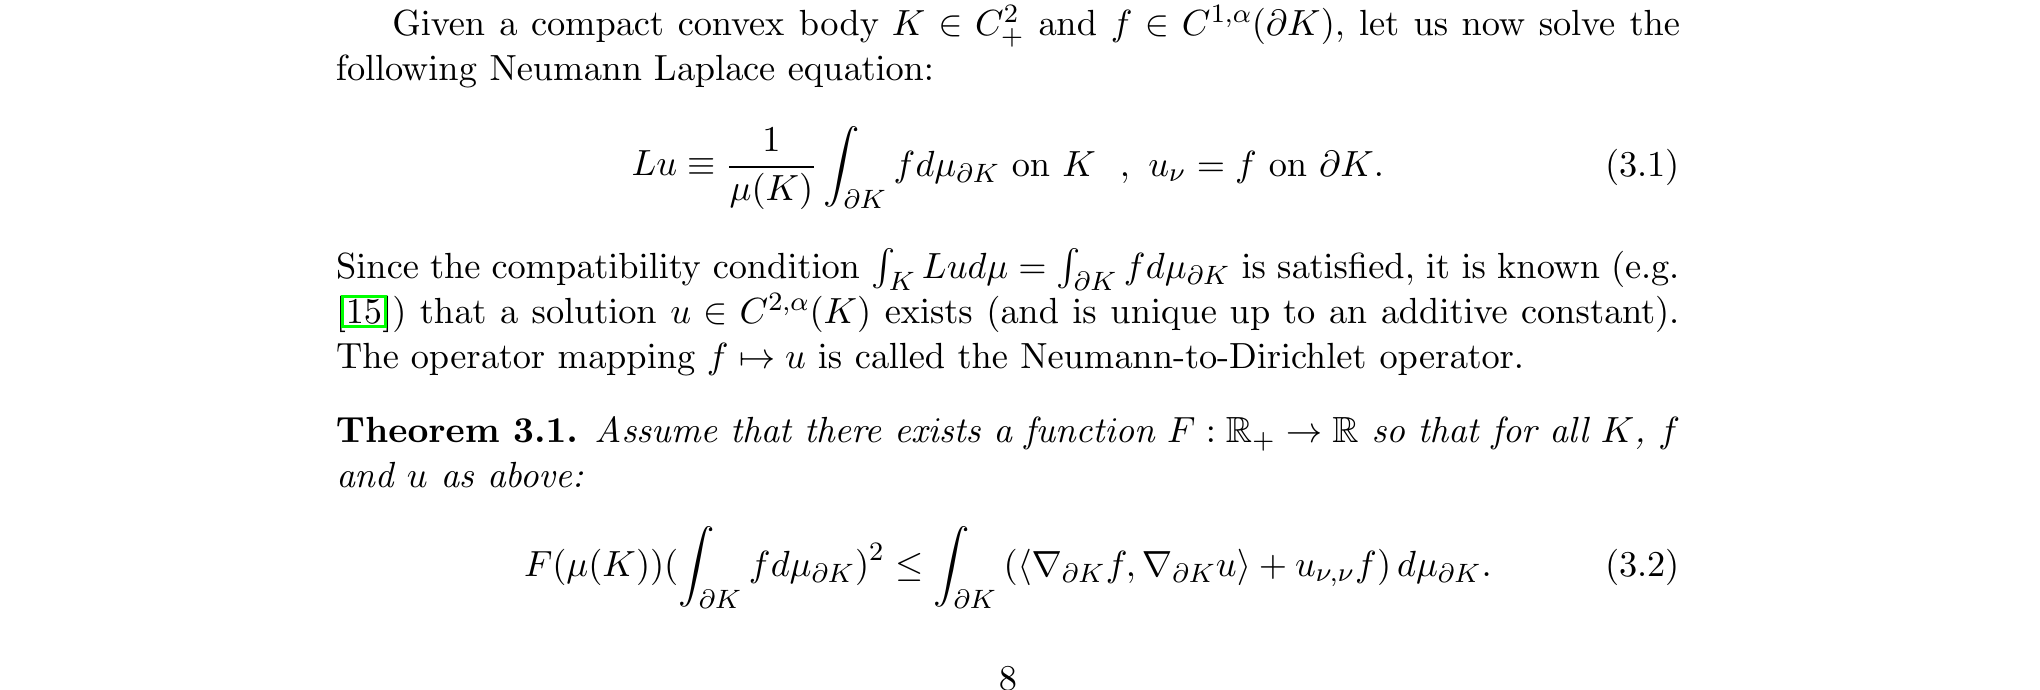
\includegraphics[width=0.98\linewidth]{figures/condition_3_2_crop.png}
\end{center}

For the standard Gaussian, Lemma 3.2 of the source identifies the right-hand
side of (3.2) with
\begin{equation}\label{eq:energy}
 \mathcal E_K(u):=\int_K
 \bigl(\|\nabla^2u\|_{\mathrm{HS}}^2+|\nabla u|^2\bigr)\,d\gamma_2.
\end{equation}
Thus, if $\cL=\Delta-\langle x,\nabla\rangle$, $\cL u=1$, and
$f=u_\nu$, condition (3.2) requires
\begin{equation}\label{eq:required}
 \mathcal E_K(u)\geq F(\gamma_2(K))\gamma_2(K)^2.
\end{equation}

\section*{Proof Intuition}

The halfspace of Gaussian measure $1/2$ is an equality case.  Its one-dimensional
solution has derivative $w=\Phi/\varphi$.  The first genuinely curved
tangential perturbation is the second Hermite mode
$\rho(y)=(1-y^2)/\sqrt2$.  Differentiation raises the positive
one-dimensional Ornstein--Uhlenbeck eigenvalue: $\cL_x w'=2w'$, while
$\cL_y\rho=-2\rho$.  Hence $w'(x)\rho(y)$ is $\cL$-harmonic and can be added
without changing the constant source $\cL u=1$.

Optimizing this correction on a volume-preserving parabolic deformation of
the halfspace produces the strictly negative coefficient
$-(4-\pi)^2/(16\pi)$.  The parabola itself is unbounded, but large ellipses
converge to it in both Gaussian volume and the energy \eqref{eq:energy}.
The strict deficit therefore survives on a finite smooth strictly convex
ellipse, which satisfies all hypotheses in the source question.

\section*{Counterexample Theorem}

\begin{theorem}\label{thm:main}
There exist a compact $C^\infty$ strictly convex body $K\subset\R^2$, a
function $u\in C^\infty(\overline K)$ satisfying $\cL u=1$ in $K$, and the
smooth Neumann datum $f=u_\nu$ on $\partial K$, such that
\[
 \gamma_2(K)=\frac12,
 \qquad
 \mathcal E_K(u)<\frac12
 =F\!\left(\frac12\right)
   \left(\int_{\partial K}f\,d\gamma_{\partial K}\right)^2.
\]
Consequently condition (3.2) in the source paper is false for the standard
Gaussian measure, and Question 3.4 has a negative answer.
\end{theorem}

\section*{Proof}

Write
\[
 \varphi(x)=\frac{1}{\sqrt{2\pi}}e^{-x^2/2},
 \qquad
 \Phi(x)=\int_{-\infty}^x\varphi(t)\,dt,
 \qquad
 w(x)=\frac{\Phi(x)}{\varphi(x)}.
\]
Then
\begin{equation}\label{eq:w-identities}
 w'=1+xw,
 \qquad \cL_xw=w,
 \qquad \cL_xw'=2w'.
\end{equation}
Choose a smooth primitive $W$ of $w$.  The first identity gives
\begin{equation}\label{eq:particular}
 \cL_xW=W''-xW'=w'-xw=1.
\end{equation}
Let
\[
 \rho(y)=\frac{1-y^2}{\sqrt2}.
\]
For a standard one-dimensional Gaussian variable $Y$,
\begin{equation}\label{eq:rho}
 \cL_y\rho=-2\rho,
 \quad
 \mathbb E\rho(Y)=0,
 \quad
 \mathbb E\rho(Y)^2=1,
 \quad
 \mathbb E\rho'(Y)^2=2.
\end{equation}
Put $a=w'$ and
\begin{equation}\label{eq:u-eps}
 u_{\eps,A}(x,y)=W(x)+\eps A a(x)\rho(y).
\end{equation}
Equations \eqref{eq:w-identities}--\eqref{eq:rho} imply
\begin{equation}\label{eq:constant-source}
 \cL u_{\eps,A}=1
\end{equation}
on all of $\R^2$.

\subsection*{The volume-preserving parabolic model}

For $\eps$ near zero, let
\[
 P_\eps=\{(x,y):x<c(\eps)+\eps\rho(y)\},
\]
where $c(\eps)$ is chosen so that $\gamma_2(P_\eps)=1/2$.  Such a unique
smooth $c(\eps)$ exists by the implicit function theorem applied to
\[
 V(c,\eps)=\mathbb E\,\Phi(c+\eps\rho(Y)).
\]
At $(c,\eps)=(0,0)$, equations \eqref{eq:rho} and
$\varphi'(0)=0$ give
\[
 V_c=\varphi(0)>0,
 \qquad V_\eps=0,
 \qquad V_{\eps\eps}=0.
\]
It follows that
\begin{equation}\label{eq:c-small}
 c(0)=c'(0)=c''(0)=0,
 \qquad c(\eps)=o(\eps^2).
\end{equation}
Since $\rho''=-\sqrt2$, the graphing function is strictly concave when
$\eps>0$, and $P_\eps$ is convex.

We now compute the energy through order $\eps^2$.  Set
\[
 q_0=w'^2+w^2,
 \qquad
 B=w'a''+wa'.
\]
Expanding the quadratic energy density of \eqref{eq:u-eps}, then expanding
the upper integration limit $c(\eps)+\eps\rho(y)$, gives
\begin{equation}\label{eq:energy-expansion}
 \mathcal E_{P_\eps}(u_{\eps,A})
 =\mathcal E_{P_0}(W)
  +\eps^2\bigl(C_0+2AL+A^2D\bigr)+o(\eps^2),
\end{equation}
where
\begin{align}
 C_0&=\frac12\varphi(0)q_0'(0)\,\mathbb E\rho^2,\label{eq:C0}\\
 L&=\varphi(0)B(0)\,\mathbb E\rho^2,\label{eq:L}\\
 D&=\int_{\{x<0\}}
 \left(\|\nabla^2(a\rho)\|_{\mathrm{HS}}^2
             +|\nabla(a\rho)|^2\right)d\gamma_2.\label{eq:D}
\end{align}
For completeness, the terms of order $\eps$ vanish because
$\mathbb E\rho=0$.  The base-density boundary shift contributes
$\frac12\varphi(0)q_0'(0)\mathbb E\rho^2$; the cross-energy boundary shift
contributes $2AL$; the interior quadratic term is $A^2D$; and
\eqref{eq:c-small} shows that the volume correction contributes only
$o(\eps^2)$.  This proves \eqref{eq:energy-expansion} directly by Taylor's
formula and Gaussian domination.

Put $\alpha=w(0)=\sqrt{\pi/2}$.  Successive differentiation of
$w'=1+xw$ gives
\begin{equation}\label{eq:origin-values}
 w(0)=\alpha,
 \qquad w'(0)=1,
 \qquad w''(0)=\alpha,
 \qquad w'''(0)=2,
 \qquad \varphi(0)\alpha=\frac12.
\end{equation}
Because $\cL_xw=w$, one-dimensional Gaussian integration by parts yields
\begin{equation}\label{eq:E0}
 \mathcal E_{P_0}(W)
 =\int_{-\infty}^0(w'^2+w^2)\varphi\,dx
 =\varphi(0)w(0)w'(0)=\frac12.
\end{equation}
Equations \eqref{eq:C0}, \eqref{eq:L}, and \eqref{eq:origin-values} give
\begin{equation}\label{eq:C0L-values}
 C_0=1,
 \qquad
 L=\varphi(0)(2+\alpha^2)
   =\frac{\pi+4}{2\sqrt{2\pi}}.
\end{equation}

It remains to evaluate $D$.  Let $\psi=a(x)\rho(y)$.  Since $\cL\psi=0$,
differentiating shows that $\cL(\partial_i\psi)=\partial_i\psi$.  Gaussian
integration by parts on the halfspace therefore gives
\begin{align*}
 D
 &=\varphi(0)\,\mathbb E\left[
       \nabla\psi(0,Y)\mathbin{\cdot}\partial_x\nabla\psi(0,Y)
     \right]\\
 &=\varphi(0)\left(
       a'(0)a''(0)\mathbb E\rho^2
       +a(0)a'(0)\mathbb E(\rho')^2
     \right).
\end{align*}
Here $a=w'$, so \eqref{eq:rho} and \eqref{eq:origin-values} yield
\begin{equation}\label{eq:D-value}
 D=\varphi(0)(2\alpha+2\alpha)=2.
\end{equation}

The quadratic coefficient in \eqref{eq:energy-expansion} is minimized at
\begin{equation}\label{eq:Aopt}
 A_*=-\frac{L}{D}=-\frac{\pi+4}{4\sqrt{2\pi}}.
\end{equation}
Using \eqref{eq:E0}, \eqref{eq:C0L-values}, and \eqref{eq:D-value}, we obtain
the exact expansion
\begin{equation}\label{eq:negative}
 \mathcal E_{P_\eps}(u_{\eps,A_*})
 =\frac12-\frac{(4-\pi)^2}{16\pi}\eps^2+o(\eps^2).
\end{equation}
In particular, this energy is strictly smaller than $1/2$ for every
sufficiently small positive $\eps$.

\subsection*{Compactification by ellipses}

Fix one such $\eps>0$.  For $R>0$ and $c\in\R$, define the ellipse
\begin{equation}\label{eq:ellipse}
 K_{\eps,R,c}=\left\{(x,y):
 \frac{(x-c-\eps/\sqrt2+R)^2}{R^2}
 +\frac{\sqrt2\eps}{R}y^2\leq1\right\}.
\end{equation}
Its right boundary is
\[
 b_{\eps,R,c}(y)=c+\frac\eps{\sqrt2}-R
 +R\sqrt{1-\frac{\sqrt2\eps}{R}y^2}.
\]
For every fixed $y$,
\begin{equation}\label{eq:boundary-limit}
 b_{\eps,R,c}(y)\longrightarrow
 c+\frac\eps{\sqrt2}-\frac\eps{\sqrt2}y^2
 =c+\eps\rho(y),
\end{equation}
while the left boundary tends to $-\infty$.

For every sufficiently large $R$, translate in the $x$ direction and choose
a local normalizing parameter $c=c_{\eps,R}$ near $c(\eps)$ such that
$\gamma_2(K_{\eps,R,c_{\eps,R}})=1/2$.  Indeed, on a fixed neighborhood of
$c(\eps)$ the volume and its $c$-derivative converge to
$V(c,\eps)$ and $V_c(c,\eps)>0$, respectively.  The implicit function theorem
therefore supplies a unique root in that neighborhood for large $R$, and
\begin{equation}\label{eq:c-limit}
 c_{\eps,R}\longrightarrow c(\eps).
\end{equation}
The same dominated-convergence argument applied to the energy density of the
fixed smooth function $u_{\eps,A_*}$ gives
\begin{equation}\label{eq:energy-limit}
 \mathcal E_{K_{\eps,R,c_{\eps,R}}}(u_{\eps,A_*})
 \longrightarrow
 \mathcal E_{P_\eps}(u_{\eps,A_*})<\frac12.
\end{equation}
To justify domination explicitly, \eqref{eq:boundary-limit} gives a uniform
upper bound on $x$; as $x\to-\infty$, the standard Mills-ratio identities
from $w'=1+xw$ give polynomial decay of $w,w',w'',w'''$; and the $y$
dependence is polynomial times the Gaussian density.  Thus the energy has an
integrable majorant independent of large $R$.

Choose a finite large $R$ for which the strict inequality in
\eqref{eq:energy-limit} holds, and write $K=K_{\eps,R,c_{\eps,R}}$.  This $K$
is compact, $C^\infty$, and has everywhere positive curvature.  Let
$u=u_{\eps,A_*}$ and $f=u_\nu$.  By \eqref{eq:constant-source} and Gaussian
integration by parts,
\begin{equation}\label{eq:flux}
 \int_{\partial K}f\,d\gamma_{\partial K}
 =\int_K\cL u\,d\gamma_2=\gamma_2(K)=\frac12.
\end{equation}
Finally, $\Phi^{-1}(1/2)=0$, so $(\log I_\gamma)'(1/2)=0$ and
$F(1/2)=2$.  Equations \eqref{eq:energy-limit} and \eqref{eq:flux} show
\[
 \mathcal E_K(u)<\frac12
 =2\left(\frac12\right)^2
 =F(\gamma_2(K))
   \left(\int_{\partial K}f\,d\gamma_{\partial K}\right)^2.
\]
This is the required violation of condition (3.2), proving
Theorem~\ref{thm:main}. \qed

\section*{Verification Notes}

The proof is analytic and does not depend on numerical quadrature.  The
included script
\texttt{code/check\_second\_variation\_and\_ellipses.py} checks the identity
\[
 1-\frac{1}{2}\left(\frac{\pi+4}{2\sqrt{2\pi}}\right)^2
 =-\frac{(4-\pi)^2}{16\pi}
\]
to floating-point precision and independently integrates finite ellipses.
For example, at $\eps=0.03$ and $R=100$, after translating to numerical
Gaussian volume $0.5$, it reports energy approximately
$0.49999660148$.  These computations are sanity checks only.

Initial reconnaissance optimized every interval on a $65$-point endpoint
grid (2016 intervals), scanned centered Gaussian balls in dimensions 2 through
10, and tested product halfspace models.  No violation appeared because the
negative mode requires both curvature and a nontrivial tangential direction.

\section*{Novelty Check and Limitations}

Before promotion, the cheap run indexes were searched for arXiv:1601.02925,
the exact source title, ``Gaussian Neumann-to-Dirichlet'', and the fixed-source
Hessian-energy formulation.  No prior solution or counterexample packet for
this question was present.

Web and arXiv searches on 2026-08-09 used the exact question title, the source
authors and arXiv id, ``Gaussian Neumann-to-Dirichlet convex domains'', and
``Gaussian Hessian energy Neumann convex''.  They found the source question
but no later paper claiming to resolve it or containing this parabolic
counterexample.  Kai-Wen Yang's 2026 paper \cite{Yang} was inspected because
it uses raywise localization of Gaussian Neumann Hessian energy.  Its argument
selects a variable source $\cL u=g$ for a different Brunn--Minkowski problem;
it does not answer the present fixed-constant-source condition.

This was a bounded rather than exhaustive novelty search.  The packet claims
a likely valid candidate counterexample, not certified publication novelty.

\section*{Human Review Recommendation}

The recommended review focus is narrow: check the Taylor expansion
\eqref{eq:energy-expansion}, especially the cross-energy boundary shift, and
check the dominated-convergence passage \eqref{eq:c-limit}--\eqref{eq:energy-limit}.
All remaining steps are explicit Ornstein--Uhlenbeck identities and Gaussian
integration by parts.

\begin{thebibliography}{9}

\bibitem{KM}
A. V. Kolesnikov and E. Milman,
\emph{Sharp Poincar\'e-type inequality for the Gaussian measure on the boundary
of convex sets}, Geometric Aspects of Functional Analysis, Lecture Notes in
Mathematics 2169, 221--234, 2017; arXiv:1601.02925.

\bibitem{Yang}
K.-W. Yang,
\emph{The Brunn--Minkowski inequality for the Gaussian measure},
arXiv:2608.05390, 2026.

\end{thebibliography}

\end{document}
